% \documentclass{article} % For LaTeX2e
% \usepackage{nips13submit_e,times}
\documentclass[UTF8]{ctexart}
\usepackage{CJK}
% \usepackage{ctex}
\usepackage{amsmath}
% \usepackage{amssymb}
\usepackage{geometry}
\usepackage{graphicx}
\usepackage{float}
% \usepackage{hyperref}
% \usepackage{url}
\usepackage{algpseudocode}
\usepackage{algorithm}
\usepackage{algorithmicx}
% \usepackage{textcomp}  % \textcelsius
% \graphicspath{{./fig/}}
\usepackage{caption,subcaption}
\usepackage{color}
\usepackage{mathtools}
\CTEXsetup[format={\Large\bfseries}]{section}
\title{Algorithm Design and Analysis: Assignment 1}
\author{钟赟 202028013229148}
\usepackage{geometry}
\geometry{left=2.5cm,right=2.5cm,top=2.5cm,bottom=2.5cm}

\newcommand{\fix}{\marginpar{FIX}}
\newcommand{\new}{\marginpar{NEW}}

\newtheorem{theorem}{Theorem}
\newtheorem{proof}{Proof}
\newtheorem{problem}{Problem}

\begin{document}
% \begin{CJK}{GBK}{song}

\maketitle

\section*{Problem 1}
Suppose an array sorted in ascending order is rotated at some pivot unknown to you be-forehand. (i.e., [0, 1, 2, 4, 5, 6, 7] is an ascending array, then it might be rotated and become
[4, 5, 6, 7, 0, 1, 2].) How to find the minimum of a rotated sorted array?
(Hint: All elements in the array are distinct.)

For example, the minimum of rotated sorted array [4, 5, 6, 7, 0, 1, 2] is 0.

Please give an algorithm with $\mathcal{O}(log n)$ complexity, prove the correctness and analyze the complexity.
\section*{Answer 1}
\subsection*{1.1 Algorithm Description} 
We consider using binary search method to solve the problem. For array [0, 1, 2, 3, 4, 5, 6, 7], there are total 7 rotated forms as follows (the red number is the median) :
\begin{center}
	[0, 1, 2, \textcolor{red}{4}, 5, 6, 7]\\{}
	[7, 0, 1, \textcolor{red}{2}, 4, 5, 6]\\{}
	[6, 7, 0, \textcolor{red}{1}, 2, 4, 5]\\{}
	[5, 6, 7, \textcolor{red}{0}, 1, 2, 4]\\{}
	[4, 5, 6, \textcolor{red}{7}, 0, 1, 2]\\{}
	[2, 4, 5, \textcolor{red}{6}, 7, 0, 1]\\{}
	[1, 2, 4, \textcolor{red}{5}, 6, 7, 0]\\{}
\end{center}

After selecting the median as a pivot, the key problem is to decide which part to search next step. We can see in the example that if the median is less than the element rightmost, the right part is sorted and the left part contains the minimum, the left part is sorted and the right part contains the minimum otherwise. 

Suppose the length of array $ A$ is $ n $. $ A[i] $ is the minimum if and only if $ A[i] == A[(i+n-1)\%n] $ -- the element before the minimum is greater than it.

Here is my algorithm. For an array $ A $ with length $ n $:

1. Select the median $A[i]$ of array $ A $ (or sub-array) as an pivot, $i = \frac{l+r}{2}$;

2. If $ A[i] == A[(+n-1)\%n] $, $ A[i] $ is the minimum. Otherwise goto step 3. ;

3. If $ A[i] < A[rightmost] $, substitute $ A $ with $ A_{LEFT} $ . Goto step 1. ; 

4. If $ A[i] > A[rightmost] $, substitute $ A $ with $ A_{RIGHT} $ . Goto step 1. \\

Pseudo-code : see \textbf{Algorithm 1}. 

\begin{algorithm}[h]
	\caption{MIN\_ROTATED\_ARRAY algorithm}
	\begin{algorithmic}[1]
		\Function{MIN\_ROTATED\_ARRAY}{$A, n, l, r$}
		\State $l = 0$;  $r = n - 1$; 
		\While{$l \leq r$}
			\State $pivot = \frac{l + r}{2}$;
			\If{$A[pivot] < A[(pivot+n-1)\%n]$}
				\State \Return{$A[pivot]$};
			\EndIf
			\If{$A[pivot] < A[r]$}
				\State $r = pivot$;
			\Else
				\State $l=pivot$;
			\EndIf
		\EndWhile
		\State \Return{$0$} ;
		\EndFunction
	\end{algorithmic}
\end{algorithm}

\subsection*{1.2 Subproblem Reduction Graph} 
Take array [6,7,0,1,2,4,5] as an example, \textbf{Graph 1} shows the procedure of finding its minimum. 

\begin{figure} [htb]
	\centering
	\caption*{Graph 1}
	% \caption*{fig1: Subproblem reduction graph of $MIN\_ROTATED\_ARRAY(A, n, l, r)$ algorithm}
	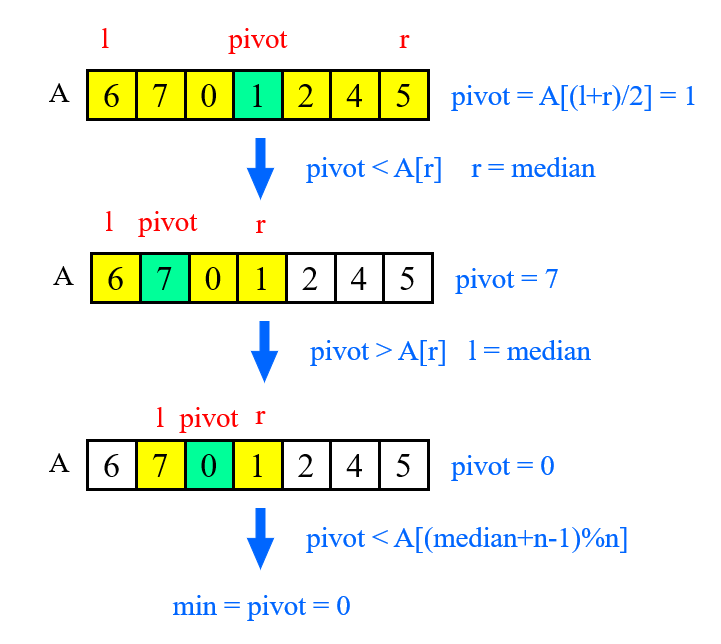
\includegraphics[width=0.5\textwidth]{figs/1.png}
\end{figure}


\subsection*{1.3 Correctness Proof } 
(1) The algorithm is clearly correct where $ n = 1 $ and $n = 2$.

(2) Assuming that the algorithm is correct in the case of $n \leq k , k \geq 2$, let's think about cases when $ n = k + 1$.

If $ A[\lfloor \frac{n}{2} \rfloor] < A[n] $ and the index of the minimum element exists in $ (\lfloor \frac{n}{2} \rfloor, n) $, 
then we have $minimum \leq A[n-1] < A[\lfloor \frac{n}{2} \rfloor]$ according to the ascending order before rotated, which results in contradiction.
Threfore the minimum element is between $A[0]$ and $A[\lfloor \frac{n}{2} \rfloor]$. After one iteration, $A' = A[0, \lfloor \frac{n}{2} \rfloor]$.
The size of $\mid A'\mid \leq [\frac{n}{2}] + 1 < k $, then we can always find the minimum by the assumption.

If $ A[\lfloor \frac{n}{2} \rfloor] > A[n] $ and the index of the minimum element is in $ [0, \lfloor \frac{n}{2} \rfloor] $, 
then we have $minimum \leq A[\lfloor \frac{n}{2} \rfloor] < A[n]$ according to the ascending order before rotated, which results in contradiction.
Threfore the minimum element is between $A[\lfloor \frac{n}{2} \rfloor]$ and $A[n-1]$. After one iteration, $A' = A[\lfloor \frac{n}{2} \rfloor, n-1]$.
The size of $\mid A'\mid \leq [\frac{n}{2}] + 1 < k $, then we can always find the minimum by the assumption.

(3) To sum up, the algorithm is correct for any array $A[n]$ with $n \geq 1$.

\subsection*{1.4 Complexity}  
The time complexity is $\mathcal{O}(log n)$ as binary search once costs time of $(logn)$.

The space complexity is $\mathcal{O}(1)$ .

\section*{Problem 2}
Consider an n-node complete binary tree $T$ , where $n = 2^d - 1$ for some $d$. Each node $v$ of
$T$ is labeled with a real number $x_v$. You may assume that the real numbers labeling the nodes
are all distinct. A node $v$ of $T$ is a local minimum if the label $x_v$ is less than the label $x_w$ for
all nodes $w$ that are joined to $v$ by an edge. 
You are given such a complete binary tree $T$ , but the labeling is only specifed in the following:
implicit way: for each node $v$, you can determine the value $x_v$ by probing the node $v$.
Show how to find a local minimum of $T$ using only $\mathcal{O}(logn)$ probes to the nodes of $T$ .

\section*{Answer 2}
\subsection*{2.1 Algorithm Description}
In order to find the local minimum, we need to compare the label $x_v$ of node $v$ and the labels for nodes joined to $v$.
Let's devide the complete binary tree $T$ into 2 subtrees when searching from the root, and the size of the subproblems decreases exponentially.
For  node $v$, if it has no children, then $ return v $; or if $x_v$ is more than the labels of $v$'s children, then $ return v $; else if $x_v$ is less than one of $v$'s child's label,
search the subtree rooted by the child with larger label recursively.\\

Pseudo-code : see \textbf{Algorithm 2}. 
\begin{algorithm}[h]
	\caption{LOCAL\_MIN\_PROBE algorithm}
	\begin{algorithmic}[1]
	\Function{LOCAL\_MIN\_PROBE}{$T, v$}
		\If{$v$ has no child}
			\State \Return{$v$};
		\EndIf
		\State $ l $ = left child of $v $;
		\State $ r$ = right child of $v $;
		\If{$x_v > x_l$ and $x_v > x_r$}
			\Return{$v$} ;
		\Else
			\State $u = $ min $(l, r)$; \Comment {$min(l, r)$ returns the node with less label}
			\State \Return{LOCAL\_MIN\_PROBE $(T, u)$}; 
		\EndIf
	\EndFunction
	\end{algorithmic}
\end{algorithm}

\subsection*{2.2 Subproblem Reduction Graph} 
See \textbf{Graph 2}.
\begin{figure} [htbp]
	\centering
	\caption*{Graph 2}
	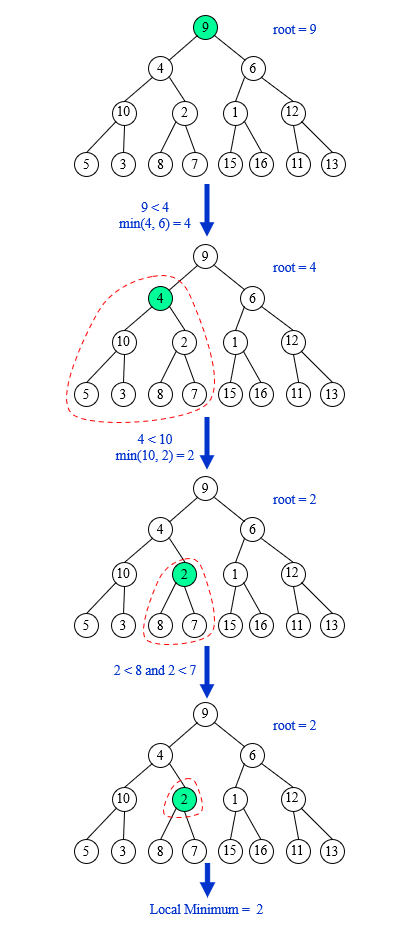
\includegraphics[width=0.5\textwidth]{figs/2.png}
\end{figure}

\subsection*{2.3 Correctness Proof} 
We already know that the number of tree $T$ is $n = 2^d-1$:

(1) When $d = 0, n = 1$, the root is the local minimum. The algorithm is clearly correct.

(2) Assuming that the algorithm is correct in the case of $d \leq k , k \geq 0$, let's think about cases when $ d = k + 1$, 
that is the depth of the tree increase by $1$.

If the label of root node is less than its children's, the root node returned by the algorithm is the local minimum.
Otherwise if its child $u$ has the smallest label, the algorithm would call LOCAL\_MIN\_PROBE$(T, u)$. The subtree $u$ 
has a depth $ < d$ and a number of nodes $\leq 2^{d-1}-1 = 2^k-1$, thus the algorithm should return the local minimum of tree $u$, say $w$, by the assumption.
If $u = w$, $w$ is clearly the local minimum of tree $T$. If $u \neq w$, $w$ is also the local minimum of tree $T$ as 
the label of $w$ is less than the labels for all nodes joined to $w$ by an edge.

(3) To sum up, the algorithm is correct for given $d \geq 0$ .

\subsection*{2.4 Complexity} 
According to the Master's Theorem, $T(n) = T(\frac{n}{2}) + 1 = \mathcal{O}(log n)$.
\section*{Problem 3}
Given an integer array, one or more consecutive integers in the array form a sub-array. Find
the maximum value of the sum of all subarrays.\\
Please give an algorithm with $\mathcal{O}(nlogn)$ complexity.
\section*{Answer 3}
\subsection*{3.1  Algorithm Description}
Similar to the algorithm used in CLOSEST\_PAIRS problem, I decide to apply DEVIDE-CONQUER-COMBINE method to this problem.

DEVIDE: dividing the array into 2 roughly equal subarrays.

CONQUER: finding the maximum value of the sum of subarrays in each half.

COMBINE: considering subarrays consisting of elements from both left half and right half, and finding the real maximum sum.

We define a function MAX\_SUM\_SUBARRAY$(A, l , r)$ to identify finding the the maximum sum of subarray $A[l,r]$. Each time we devide interval $[l,r]$ into 2 halves by 
$m = \lfloor \frac{l+r}{2} \rfloor$, and implement CONQUER in $A[l, m]$ and $A[m+1, r]$, respectively. When the length of intervals are reduced to 1, we start to COMBINE information 
of $A[l, m]$ and $A[m+1, r]$.

Some extra variants are needed to store information of subarrays:

$imax$: sum of all elements in $A[l,r]$;

$lmax$: the maximum sum of subarrays of $A[l,r]$ with $A[l]$ as the left endpoint;

$rmax$: the maximum sum of subarrays of $A[l,r]$ with $A[r]$ as the right endpoint;

$mmax$: the maximum sum of subarrays of $A[l,r]$.

While combining information, the variants iterate like this:

$imax_{[l,r]} = imax_{[l,m]} + imax_{[m+1,r]}$;

$lmax_{[l,r]} = $MAX$(lmax_{[l,r]}, imax_{[l,m]} + lmax_{[m+1,r]})$;

$rmax_{[l,r]} = $MAX$(rmax_{[l,r]}, rmax_{[l,m]} + imax_{[m+1,r]})$;

$mmax_{[l,r]} = $MAX$($MAX$(mmax_{[l,m]}, mmax_{[m+1,r]}), rmax_{[l,m]} + lmax_{[m+1,r]})$;

After combining all subarrays into the whole array, the $mmax_{[0,n-1]}$ returns the maximum sum of subarrays of $A$.\\

Pseudo-code : see \textbf{Agorithm 3}.

\begin{algorithm}[h]
	\caption{MAX\_SUM\_SUBARRAYS algorithm}
	\begin{algorithmic}[1]
		\Function{MAX\_SUM\_SUBARRAY}{$A, l , r$}
		\While{$l < r$}
			\State $m = \lfloor \frac{l+r}{2} \rfloor$; \Comment{DIVIDE procedure}
			\State $\{imax_l, lmax_l, rmax_l, mmax_l\} =  $MAX\_SUM\_SUBARRAY$(A, l , m)$; \Comment{CONQUER}
			\State $\{imax_r, lmax_r, rmax_r, mmax_r\} =  $MAX\_SUM\_SUBARRAY$(A, m+1 , r)$;
			\State $imax = imax_l + imax_r;$
			\State $lmax = $MAX$(lmax_l, imax_l + lmax_r);$ \Comment{COMBINE procedure}
			\State $rmax = $MAX$(rmax_r, rmax_l + imax_r);$\Comment{MAX$(a, b)$ returns the larger number of $a$ and $b$}
			\State $mmax = $MAX$($MAX$(mmax_l, rmax_r), rmax_l + lmax_r)$;
			\State \Return{$\{ imax, lmax, rmax, mmax\}$} ;
		\EndWhile
		\EndFunction
		\Function{MAX\_SUM\_SUBARRAYS}{$A$}
		\State \Return{MAX\_SUM\_SUBARRAY$(A, 0, n)$};
		\EndFunction
	\end{algorithmic}
\end{algorithm}

\subsection*{3.2 Subproblem reduction graph} 
Take array [-2, 1, -3, 4, -1, 2, 1] as an example, the subproblem reduction graph is seen in \textbf{Graph 3}.

\begin{figure} [h]
	\centering
	\caption*{Graph 3}
	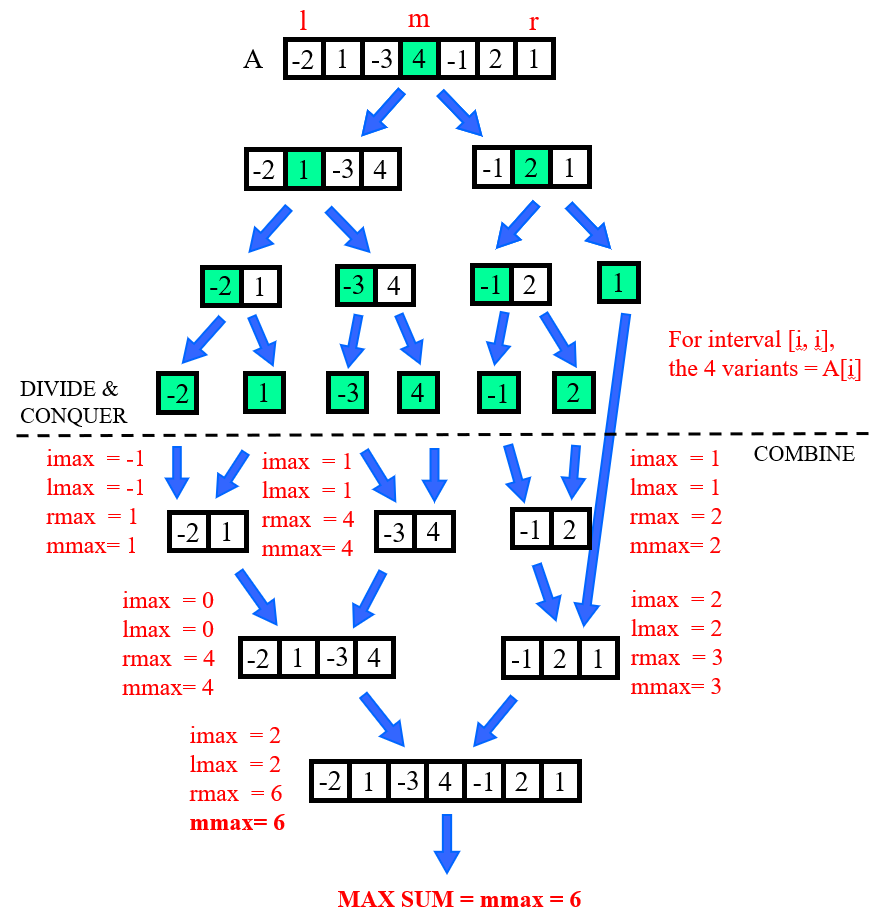
\includegraphics[width=0.8\textwidth]{figs/3.png}
\end{figure}

\subsection*{3.3 Correctness Proof} 
(1) Suppose array $A$ has length of $n$. The algorithm returns $A[0]$ where $ n = 1$, which is clearly correct.

(2) We assume that the algorithm is correct in case of $n \leq k$ , $k\geq 1$, and then consider cases of $n = k + 1$.

The algorithm firstly devide $A$ into 2 subarrays -- $A[0, \lfloor \frac{n}{2} \rfloor]$ and $A[\lfloor \frac{n}{2} \rfloor + 1, n-1]$, 
and MAX\_SUM\_SUBARRAY$(A,  0, \lfloor \frac{n}{2} \rfloor)$ and MAX\_SUM\_SUBARRAY$(A,  \lfloor \frac{n}{2} \rfloor, n-1)$ returns the 
maximum sum of their subarrays respectively by the assumption, denoted as $lmax_l, rmax_l, mmax_l$ and $lmax_r, rmax_r, mmax_r$. 
Then we have $mmax_{total} = $ MAX $( $MAX$ (mmax_l, rmax_r), rmax_l + lmax_r)$. The subarray of $A$ with maximum sum lies in either one of the subarrays or 
both halves, therefore the algorithm guarantees $mmax_{total}$ to be the maximum sum of $A$'s subarrays.

(3) To sum up, the algorithm is correct.
\subsection*{3.4 Complexity} 
Time complexity: $T(n) = 2T(\frac{n}{2}) + \mathcal{O}(1) = \mathcal{O}(n)$

Space complexity: $\mathcal{O}(logn)$.
\section*{Problem 4}
Given an array of integers nums sorted in ascending order, find the starting and ending
position of a given target value. If the target is not found in the array, return [-1, -1]. For
example, if the array is [5, 7, 7, 8, 8, 10] and the target is 8, then the output should be [3, 4].\\
Your algorithm's runtime complexity must be in the order of $\mathcal{O}(log n)$, prove the correctness
and analyze the complexity.

\section*{Answer 4}
\subsection*{4.1 Algorithm Description}
We consider finding the target value via binary search since the array is sorted. Now we have to deal with the cases of
$pivot = target$, when the starting position and ending position of the target exist in either side of the pivot. Therefore, we have to search left and right 
, respectively. If we aim to get the starting position, searching in the left subarray; searching in the right subarray for ending position otherwise.\\

Pseudo-code : see \textbf{Algorithm 4}. 

\begin{algorithm}[h]
	\caption{SEARCH\_FOR\_RANGE algorithm}
	\begin{algorithmic}[1]
	\Function{SEARCH\_FOR\_INDEX}{$(A, target, direction)$}
		\State $lo = 0;\quad hi = A.length;$ 
		\While{$lo < hi$}
			\State $mid = \lfloor \frac{lo+hi}{2}\rfloor$;
			\If{$A[mid] > target$} 
				\State $hi = mid$;\Comment{Binary search}
			\Else
				\State $lo = mid + 1$;
			\EndIf
			\If{$A[mid] == target$} 
				\If{$direction == "left"$} 
					\State $hi = mid;$\Comment{Search for the starting position}
				\Else  
					\State $lo = mid + 1$;\Comment{Search for the ending position}
				\EndIf
			\EndIf
		\EndWhile
		\State \Return{$lo$} ;
	\EndFunction
	\Function{SEARCH\_FOR\_RANGE}{$(A, target)$}
		\State $starting\_position = SEARCH\_FOR\_RANGE(A, target, "left")$;
		\State $ending\_position = SEARCH\_FOR\_RANGE(A, target, "right") - 1 $;
		\If{$A[starting\_position] \neq target$}
			\State \Return{$[-1, -1]$};
		\Else
			\State \Return{$[starting\_position, ending\_position]$};
		\EndIf
	\EndFunction
	\end{algorithmic}
\end{algorithm}

\subsection*{4.2 Subproblem Reduction Graph} 
See \textbf{Graph 4}.
\begin{figure} [htbp]
	\centering
	\caption*{Graph 4}
	% \caption*{fig4: Subproblem reduction graph of $ $ algorithm}
	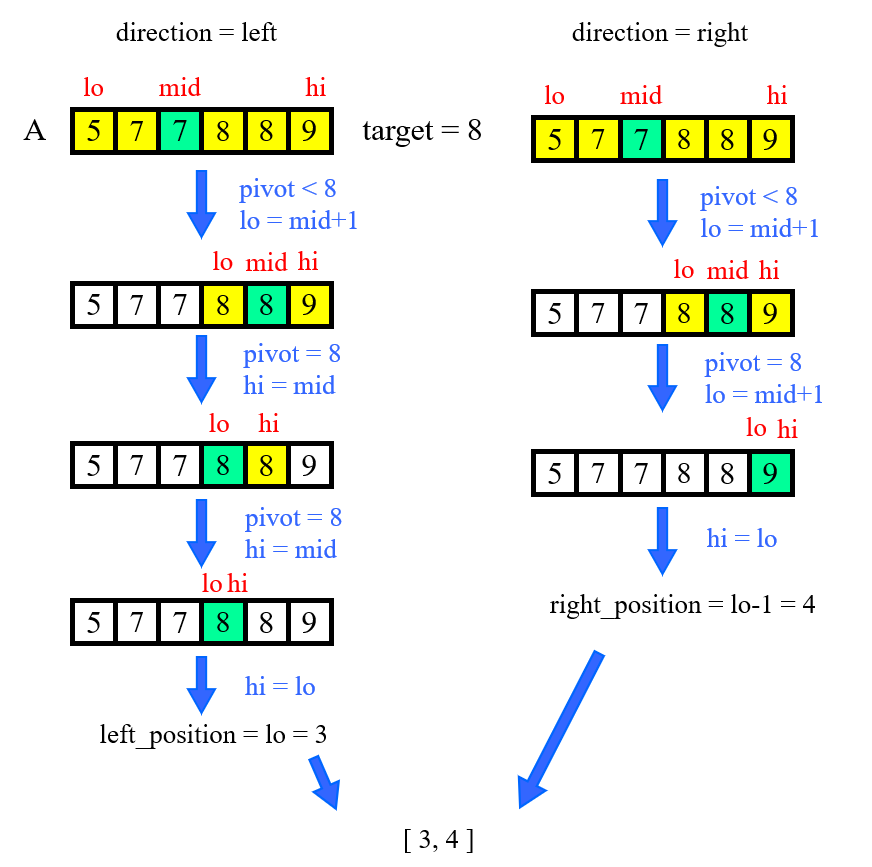
\includegraphics[width=0.8\textwidth]{figs/4.png}
\end{figure}
\subsection*{4.3 Correctness Proof} 
(1) Suppose array $A$ has length of $n$. The algorithm returns $[0, 0]$, where $ n = 1$, which is clearly correct.

(2) We assume that the algorithm is correct in case of $n \leq k$ , $k\geq 1$, and then consider cases of $n = k + 1$.

If $A[\lfloor \frac{n}{2}\rfloor] \geq target$, the starting position of target, if exists, must be in $A[0, \lfloor \frac{n}{2}\rfloor]$. The algorithm would
return the starting position of target by calling SEARCH\_FOR\_RANGE $(A', target, "left")$ , where $A' = A[0, \lfloor \frac{n}{2}\rfloor]$ with length $\lfloor \frac{n}{2}\rfloor + 1 < k$.
Then we get the starting index of the target or $-1$.

In the same way, if $A[\lfloor \frac{n}{2}\rfloor] < target$, the starting position of target, if exists, must be in $A[\lfloor \frac{n}{2}\rfloor+1, n-1]$. The algorithm would
return the starting position of target by calling SEARCH\_FOR\_RANGE $(A', target, "right")$, where $A' = A[\lfloor \frac{n}{2}\rfloor+1, n-1]$ with length $n - \lfloor \frac{n}{2}\rfloor - 2 < k$.
Then we get the starting index of the target or $-1$.

Therefore, the algorithm returns the right results when $n = k + 1$.

(3) To sum up, the algorithm is correct.
\subsection*{4.4 Complexity} 
Since binary search once costs time of $\mathcal{O}(logn)$ and the algorithm calls binary search twice, the total time complexity is $\mathcal{O}(logn)$.

Space complexity is $\mathcal{O}(1)$.

\section*{Problem 5}
Given a convex polygon with $n$ vertices, we can divide it into several separated pieces, such
that every piece is a triangle. When $n = 4$, there are two different ways to divide the polygon;
When $n = 5$, there are five different ways.\\
Give an algorithm that decides how many ways we can divide a convex polygon with $n$ vertices into triangles.

\section*{Answer 5}
\subsection*{5.1 Algorithm Description}
The simplest case: a 3-vertice convex polygon has 1 different way to be divided. For each $n$-vertice convex polygon $P$, we consider deviding it into two sub-convex polygon, and recursively dividing until into the simplest cases.
Let $d(n)$ indicate the number of ways that an n-vertice convex polygon has. 
Suppose polygon $P$ has vertices $v_1, v_2, \ldots, v_n$ and edges $(v_i, v_j), i,j = 1, 2, \ldots, n; i \neq j$. Select a vertice $v_k$ randomly, $k\in [2, n-1]$, add an edge $(v_1, v_k)$ and $(v_n, v_k)$ that
divide $P$ into a $k$-vertice convex polygon and a $n-k+1$-vertice convex polygon. For each $k$, $P$ has $d(k) * d(n-k+1)$ different ways. So $P$ has totally
$\sum_{k=2}^{n-1} d(k) * d(n-k+1)$ different ways.\\

Pseudo-code : see \textbf{Algorithm 5}. We only display one iteration of the loop of a pentagon.

\begin{algorithm}[htbp]
	\caption{CONVEX-POLYGON-DIVIDING algorithm}
	\begin{algorithmic}[1]
	\Function{CONVEX-POLYGON-DIVIDING}{$P$}
		\State $P$ has $n$ vertice;
		\State $d[2] = 1$; $d[3] = 1$;
		\For{$k = 2$ to $n-1$}
			\State $d[n] += d[k] * d[n-k+1]$;
		\EndFor
		\State \Return{$d[n]$};
	\EndFunction
	\end{algorithmic}
\end{algorithm}

\subsection*{5.2 Subproblem Reduction Graph} 
See \textbf{Graph 5}.
\begin{figure} [htb]
	\centering
	\caption*{Graph 5}
	% \caption*{fig5: Subproblem reduction graph of $ $ algorithm}
	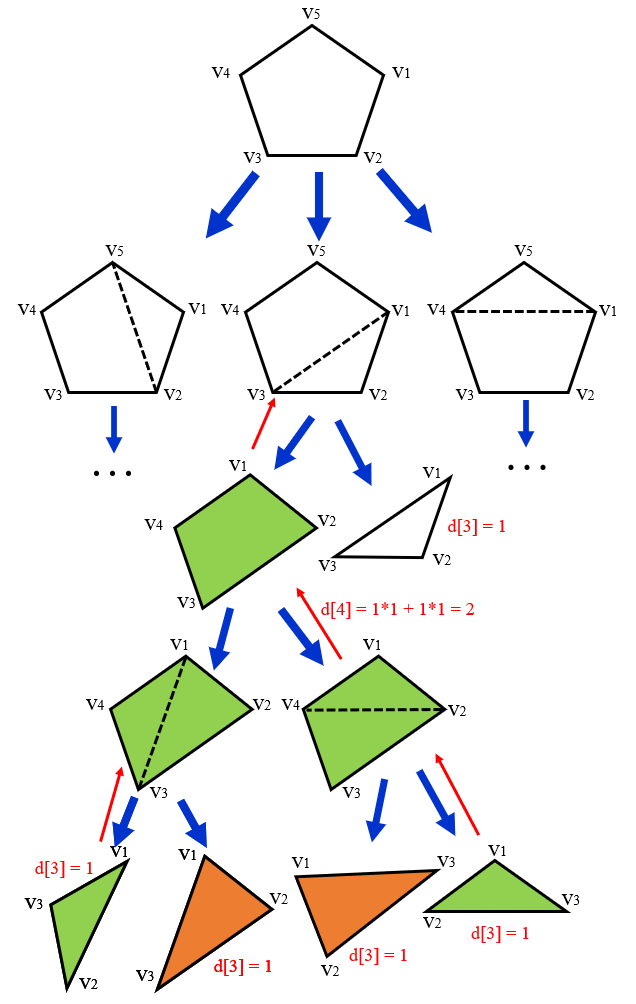
\includegraphics[width=0.8\textwidth]{figs/5.png}
\end{figure}

\subsection*{5.3 Correctness Proof} 
(1) The algorithm is clearly correct when $n = 3$;

(2) We assume that the algorithm is correct in case of $n \leq k$ , $k\geq 1$, and then consider cases of $n = k + 1$.

Supposing that the convex polygon has vertices $v_1, v_2, \ldots, v_{k+1}$. Choose a vertice $v_s$ randomly, $s \in [2, k]$. The triangle with vertices $v_1, v_{k+1}$ and $v_s$
devides the convex polygon into two parts: a polygon containing edge $(v_1, v_s)$ and a polygon containing edge $(v_{k+1}, v_s)$, thus $d(k+1) = \sum_{i=2}^{k} d(i) * d(k-i+2)$. 
Since $i \leq k$ and $k-i+2 \leq k$ for $i = 2, \ldots, k$, $d[i]$ and $d[k-i+2]$ are right computed by the assumption. Therefore the algorithm returns the correct result when $n = k+1$. 

(3) To sum up, the algorithm is correct for $n \geq 3$.
\subsection*{5.4 Complexity}
The algorithm checks all possible edges of the convex polygon, therefore its time complexity is $\mathcal{O}(n^2)$. 

\section*{Problem 6}
Recall the problem of nding the number of inversions. As in the course, we are given a
sequence of $n$ numbers $a_1, \ldots , a_n$, which we assume are all distinct, and we define an inversion
to be a pair $i < j$ such that $a_i < a_j$.

We motivated the problem of counting inversions as a good measure of how different two
orderings are. However, one might feel that this measure is too sensitive. Let's call a pair a
significant inversion if $i < j$ and $a_i > 3a_j$. Given an $O(n log n)$ algorithm to count the number
of significant inversions between two orderings.

\section*{Answer 6}
\subsection*{6.1 Algorithm Description}
Since a significant inversion requires $i < j$ and $a_i > 3a_j$, we cannot count the number of significant inversions 
while $MERGE-SORT$. Based on the $INVERSION-COUNTING$ algorithm in the course, we only need an extra counting procedure 
for 2 sorted arrays in $\mathcal{O}(n)$ time.\\

The pseudo-code is shown in \textbf{Algorithm 6}.
\begin{algorithm}[htbp]
	\caption{SIGNIFICANT-INVERSION-COUNTING algorithm}
	\begin{algorithmic}[1]
	\Function{SORT-AND-COUNT-INVERSION}{$A$}
		\If{$\parallel A \parallel$ == 1}
			\State \Return{};
		\EndIf
		\State Divide $A$ into 2 sub-sequences $L$ and $R$;
		\State $(RC_L, L)$ = SORT-AND-COUNT-INVERSION($L$);
		\State $(RC_R, R)$ = SORT-AND-COUNT-INVERSION($R$);
		\State $(C, A)$ = MERGE($L, R$);
		\State \Return{$(RC = RC_L + RC_R + C, A)$};
	\EndFunction
	\Function{MERGE}{$L, R$}
	\State $i = 0$; $j = 0$;
	\State $RC$ = COUNT-SIGNIFICANT-INVERSION($L, R, A$);
	\For{$k = 0$ to $\parallel L \parallel + \parallel R \parallel -1$ }
		\If{$L[i] > R[j]$}
			\State $A[k] = R[j]$;
			\State $j++$;
		\Else
			\State $A[k] = L[i]$;
			\State $i++$;
		\EndIf
	\EndFor
	\State \Return{$(RC, A)$};
	\EndFunction
	\Function{COUNT-SIGNIFICANT-INVERSION}{$L, R$}
		\State $RC = 0$;$i = 0$; $j = 0$;
		\While{$i < \parallel L \parallel $ and $j < \parallel R \parallel$}
			\If{$L[i] > 3 * R[j]$}
			\State $RC += (\parallel L \parallel - i)$;
			\State $j ++$;
			\Else
				\State $j++$;
			\EndIf
		\EndWhile
	\EndFunction
	
	\end{algorithmic}
\end{algorithm}

\subsection*{6.2 Subproblem Reduction Graph} 
See \textbf{Graph 6}.
\begin{figure} [htb]
	\centering
	\caption*{Graph 6}
	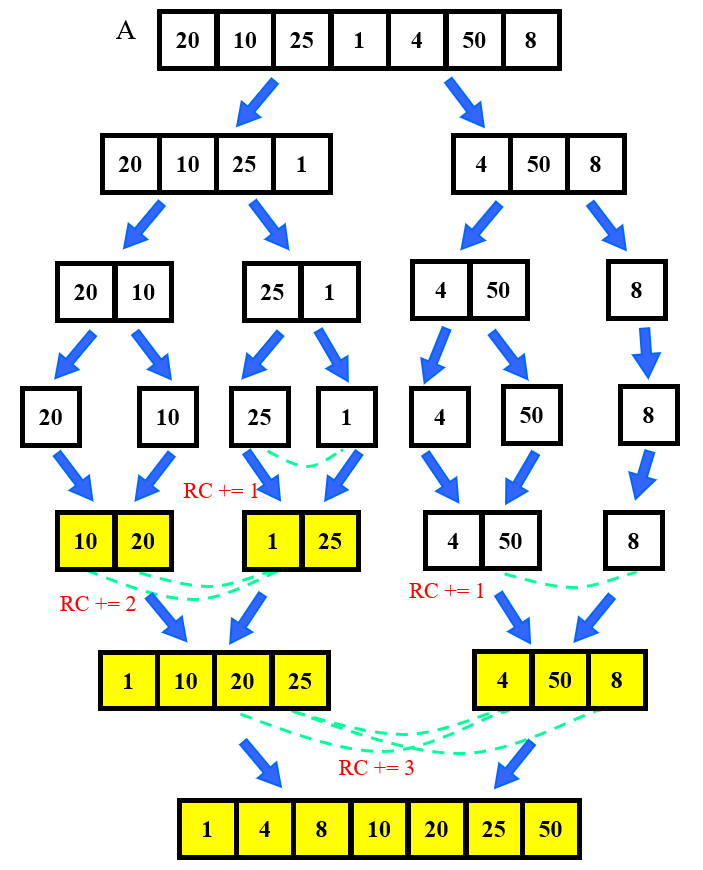
\includegraphics[width=0.6\textwidth]{figs/6.png}
\end{figure}

\subsection*{6.3 Correctness Proof} 
The algorithm, based on MERGE-SORT algorithm in the course, adds an extra function COUNT-SIGNIFICANT-INVERSION to 
count number of significant inversions. For any two sorted arrays, itetating through the arrays and doing comparisons do not 
change the structure of the array, therefore it does not change the correctness of the algorithm.
\subsection*{6.4 Complexity} 
According to the Master's Theorem, $T(n) = 2T(\frac{n}{2}) + cn = \mathcal{O}(n logn)$. 

% \end{CJK}
\end{document}
